\documentclass[11pt]{article}

\usepackage{amsmath,amssymb,amsfonts}
\usepackage{dsfont}
\usepackage{listings}
\usepackage{xcolor}
\usepackage{graphicx}
\usepackage{bbm}
\usepackage{float}


\definecolor{codegreen}{rgb}{0,0.6,0}
\definecolor{codegray}{rgb}{0.5,0.5,0.5}
\definecolor{codepurple}{rgb}{0.58,0,0.82}
\definecolor{backcolour}{rgb}{0.95,0.95,0.92}
\lstdefinestyle{mystyle}{
    backgroundcolor=\color{backcolour},   
    commentstyle=\color{codegreen},
    keywordstyle=\color{magenta},
    numberstyle=\tiny\color{codegray},
    stringstyle=\color{codepurple},
    basicstyle=\ttfamily\footnotesize,
    breakatwhitespace=false,         
    breaklines=true,                 
    captionpos=b,                    
    keepspaces=true,                 
    numbers=left,                    
    numbersep=5pt,                  
    showspaces=false,                
    showstringspaces=false,
    showtabs=false,                  
    tabsize=2
}

\setlength{\topmargin}{-.5in} \setlength{\textheight}{9.25in}
\setlength{\oddsidemargin}{0in} \setlength{\textwidth}{6.8in}

%\newcommand*{\SOLVE}{}%

\renewcommand{\vec}[1]{\mbox{\boldmath$#1$}}
\newcommand{\mm}[1]{\mathbf{#1}}

\newcounter{ProblemNum}
\newcounter{SubProblemNum}[ProblemNum]

\renewcommand{\theProblemNum}{\arabic{ProblemNum}}
\renewcommand{\theSubProblemNum}{\alph{SubProblemNum}}

\newcommand*{\anyproblem}[1]{\section*{#1}}
\newcommand*{\problem}[1]{\stepcounter{ProblemNum} %
   \anyproblem{Problem \theProblemNum \; (#1 points)}}
\newcommand*{\soln}[1]{\subsection*{#1}}
\newcommand*{\solution}{\soln{Solution}}
\newenvironment{solutions}
  {\section[Solution]{\textcolor{red}{Solution}}\color{red}}
  {\normalcolor}
\renewcommand*{\part}{\stepcounter{SubProblemNum} %
  \soln{Part (\theSubProblemNum)}}
\renewcommand{\theenumi}{(\alph{enumi})}
\renewcommand{\labelenumi}{\theenumi}
\renewcommand{\theenumii}{\roman{enumii}}
\let\endsection\relax
\let\endsubsection\relax

\graphicspath{
{.}
}
\lstset{style=mystyle}

\begin{document}

\Large
\noindent{\bf CS4851/6851 IDL: Homework 1 \hfill \today}
\medskip\hrule

\vspace{20pt}
This assignment involves implementing Perceptron algorithm in Python and testing it on various datasets. The training and test data sets will be uploaded in Moodle. Study how to use Jupyter notebook, scikit, numpy, scipy and matplotlib. Write a general python code that works for every dataset rather than different codes. Submit the executed code in Jupyter notebook. You can write your observations and results using the heading and markdown cells in Jupyter.

\vspace{20pt}
1. Implement Perceptron algorithm in Python from scratch on the datasets 

\begin{enumerate}
\item   Find the decision boundary using Perceptron algorithm on training data and plot it as shown in Figure 1
\begin{figure}[h]
    \centering
    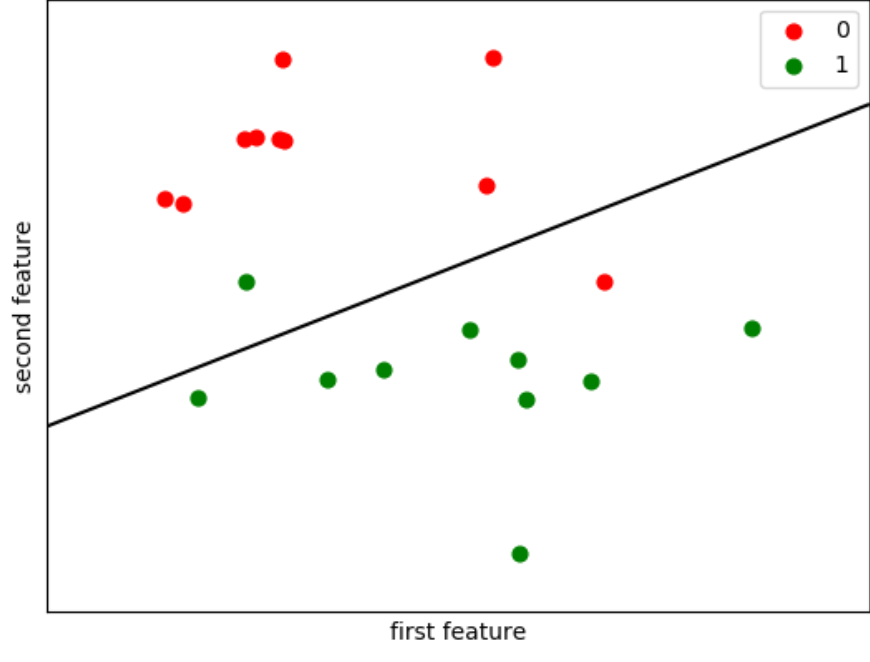
\includegraphics[width=0.8\textwidth]{Classification.png}
    \caption{Figure 1: Classification}
\end{figure}
\item Classify test data and plot the classification results.
\item Observe the weights obtained and the features of the dataset and report your findings.
\end{enumerate}
\end{document}



%%% Local Variables:
%%% mode: latex
%%% TeX-master: t
%%% End:
